\chapter{密钥分配与消息认证码的实现}
本章首先讨论数据认证机制中的密钥分配方案,以及认证过程中使用的消息认证码的实现。在6.1中基于单向hash链的思想,设计实现了面向数据认证机制的密钥分配方案。在6.2节中设计了适应无线传感网认证需求的MAC码。

\section{面向数据认证的密钥分配方案}
在本节中我们讨论研究单向hash链的性质,并将其应用到密钥分配中,设计基于单向hash链的的密钥分配机制。

我们对本章中出现的符号的定义如表~\ref{tab:macnotation}所示:
\begin{table}[htb]
  \centering
  \begin{minipage}[t]{0.8\linewidth} % 如果想在表格中使用脚注,minipage是个不错的办法
  \caption[消息认证码相关符号定义]{相关符号定义}
  \label{tab:macnotation}
    \begin{tabular*}{\linewidth}{lp{10cm}}
      \toprule[1.5pt]
      {\hei 符号} & {\hei 描述} \\
      \midrule[1pt]
      $|\mathbf{K}|$ & K的长度 \\
      $<i>$ & 表示将整数$i$用$b$位二进制表示\\
      $\mathbf{A}\|\mathbf{B}$ & 将字符串A与B进行串联 \\
      $E_K(M)$ & 对消息M使用密钥K进行分组密码置换\\
      $A\ll i$ & 将字符串A左移i位,右边填0\\
      $\mathbf{A} \oplus \mathbf{B}$ & 将字符串A与字符串B按位异或\\
      \bottomrule[1.5pt]
    \end{tabular*}
  \end{minipage}
\end{table}
\subsection{单向hash链}
本节中的密钥分配方案是基于单向hash函数的特性来保证无线传感网中的密钥安全的。通过使用单向hash链生成密钥池,能保证在密钥部署时的安全需求,还可以通过建立节点间的通信密钥有效防止攻击者通过身份冒充对节点间通信攻击。我们对单向hash链的定义以及本文方案中选取的单向hash函数进行说明。
\subsubsection{单向hash链的定义}
hash函数是通过压缩映射将任意长度的消息压缩为一个固定长度的摘要的函数。
对一个任意大小的消息,hash函数能输出一个给定长度的散列值,一个hash函数$H$可以表示为$H:\{0,1\}^*\rightarrow\{0,1\}^i$,其中$i$ 为输出的散列值的长度。
满足下列条件的hash函数称作单向hash函数:
\begin{enumerate}\setlength{\itemsep}{-\itemsep}
  \item hash函数$H(x)$的输入$x$为任意长度
  \item hash函数$H(x)$的输出为给定长度
  \item hash函数$H(x)$的计算方便,也就是对于一个给定的输入$x$,hash值输入$y=H(x)$的计算是方便的
  \item 对于给定的hash值$y=H(x)$,找出$x$在计算上是不可行的
  \item 对于给定的输入$x$,找出另一个消息$x^{'}\neq x$,满足$H(x^{'})=H(x)$在计算上是不可行的
  \item 找出任意两个消息$x$和$y$,满足$H(x)=H(y)$在计算上是不可行的,也就是$H(x)$具有抗碰撞性
\end{enumerate}



通过对一个字符串种子$K_0$使用hash函数进行迭代,形成一个字符串链,称作hash链。如果使用的hash函数是单向hash函数,则hash链称作单向hash链,链中的字符串具有不可逆计算的特性。
例如对于单向hash函数$H(x)$,通过$K_{i+1}=H(K_i),0\leq i < n$迭代生成的单向链$K_0,K_1,\cdots,K_n$就是一个单向hash链。

\subsubsection{单向hash函数的选择}
典型的单向hash函数有SHA-1或者RC5等,可以通过将算法简化,使之适应无线传感网的需求。
在SHA-1方案中,输入是最大$2^{64}$bit的消息,输出是固定160bit的消息摘要。
我们的方案中将SHA-1的输出改进为64bit(也就是我们的数据认证机制中的密钥长度),作为我们的单向hash链生成函数。

改进后的基于SHA-1 的单向hash函数算法可以表示为算法~\ref{alg:sha-1}:
\begin{algorithm}[htbp]
  \caption{单向hash函数}
  \label{alg:sha-1}
  \begin{algorithmic}[1]
    \REQUIRE 输入消息$x,|x|=64$
    \ENSURE 消息摘要
    \STATE $M \leftarrow x\| 1\| 0^t\| <|x|>$,将消息x填充为512位
    \STATE 将消息M分隔为$w_0,w_1,\cdots,w_{15}$
    \STATE $A \leftarrow h_0 = 0x67452301$
    \STATE $B \leftarrow h_1 = 0xEFCDAB89$
    \STATE $C \leftarrow h_2 = 0x98BADCFE$
    \STATE $D \leftarrow h_3 = 0x10325476$
    \STATE $E \leftarrow h_4 = 0xC3D2E1F0$
    \FOR{$i=16$ to $79$}
        \STATE $w_i \leftarrow (w_{i-3}\oplus w_{i-8}\oplus w_{i-14}\oplus w_{i-16})\ll 1$
    \ENDFOR
    \FOR{$i=0$ to $79$}
        \STATE $temp \leftarrow A\ll 5 + f(B,C,D)+E+w_i+K_i$
        \STATE $E \leftarrow D$
        \STATE $D \leftarrow C$
        \STATE $C \leftarrow B\ll 30$
        \STATE $B \leftarrow A$
        \STATE $A \leftarrow temp$
    \ENDFOR
    \STATE $A \leftarrow h_0+A$
    \STATE $C \leftarrow h_2+C$
    \RETURN $A||C$
  \end{algorithmic}
\end{algorithm}

\subsection{基于单向hash链的密钥分配}
在第四章中已经简要介绍了多路径抗节点失效中的密钥分配,在这节中对我们的基于单向hash链的密钥分配方案进行详细论述。主要分为四个部分,分别是密钥预分配、共享密钥发现、路径密钥发现和密钥分配的扩展性。
\subsubsection{密钥预分配}
在传感器节点被部署到目标监测区域之前,每个节点预先装配了足够了密钥材料,包括节点的ID信息,以及单向hash函数H(在上节中已经详细论述)。基站基于单向hash函数H生成预分配密钥池:
\begin{equation}
  K_{i,j}=H^{1}(K_{i-1,j})=\cdots=H^{i}(K_{0,j})\quad (i=1,2,\cdots,n)
\end{equation}

其中$j$为单向hash链的序号,$n$代表单条hash链中的密钥个数,$H^{i}(K_{0,j})$代表密钥$K_{0,j}$经过$i$次hash函数的迭代。
将每条hash链上的密钥反序排列,得到的hash链序列为$K_{i,j},\cdots,K_{1,j},K_{0,j}$。基站共生成$m$条单向hash链作为密钥池,则整个预分配密钥池可以如表~\ref{tab:hashline}表示:

\begin{table}[htb]
  \centering
  \begin{minipage}[t]{0.8\linewidth} % 如果想在表格中使用脚注,minipage是个不错的办法
  \caption[预分配密钥池]{预分配密钥池}
  \label{tab:hashline}
    \begin{tabular*}{\linewidth}{c}
      \toprule[1.5pt]
        $\quad \quad K_{n,1}\quad -\quad K_{n-1,1}\quad -\quad \cdots\quad -\quad K_{2,1}\quad -\quad K_{1,1}\quad -\quad K_{0,1}$\\
        $\quad \quad K_{n,2}\quad -\quad K_{n-1,2}\quad -\quad \cdots\quad -\quad K_{2,2}\quad -\quad K_{1,2}\quad -\quad K_{0,2}$\\
        $\quad \quad K_{n,3}\quad -\quad K_{n-1,3}\quad -\quad \cdots\quad -\quad K_{2,3}\quad -\quad K_{1,3}\quad -\quad K_{0,3}$\\
        $\quad \quad \cdots$\\
        $\quad \quad K_{n,m}\quad -\quad K_{n-1,m}\quad -\quad \cdots\quad -\quad K_{2,m}\quad -\quad K_{1,m}\quad -\quad K_{0,m}$\\
      \bottomrule[1.5pt]
    \end{tabular*}
  \end{minipage}
\end{table}

部署节点时,预分配的密钥从密钥池中取出,分配给节点。最先被分配的密钥是密钥池中靠前的密钥集合,也即密钥集合$K_{n,1},K_{n,2},K_{n,3},\cdots,K_{n,m}$最先被分配,后续部署到无线传感网中的节点依次从预分配密钥池中取出密钥集合进行分配。通过这样的预分配方式,不同阶段部署的节点使用的不同的密钥集合中的密钥,限制了被攻击节点泄露的密钥对整个无线传感网的影响,攻击者不能对已经建立的安全通信链路进行攻击。由于密钥池是一系列的反序单向hash 链,单向hash链的特性决定了泄露的密钥无法推导出密钥池中的密钥,因此攻击者无法进行节点冒充攻击。

\subsubsection{共享密钥发现}
节点被部署到目标区域以后,利用相应的分簇算法,对网络结构进行组织,选举每个簇的簇头。在簇的建立完成以后,节点之间开始共享密钥发现的过程。

在第二章中,我们已经讨论过密钥预分配方案的缺点,当节点被攻击而成为妥协节点时,节点中的预分配密钥都会被攻击者获得,可以对无线传感网的通信进行攻击。因此我们需要在节点之间发现相同的预分配密钥,并生成节点对之间的共享密钥。建立共享密钥的过程如图~\ref{fig:keyACK}所示:
\begin{figure}[htbp]
  \centering
  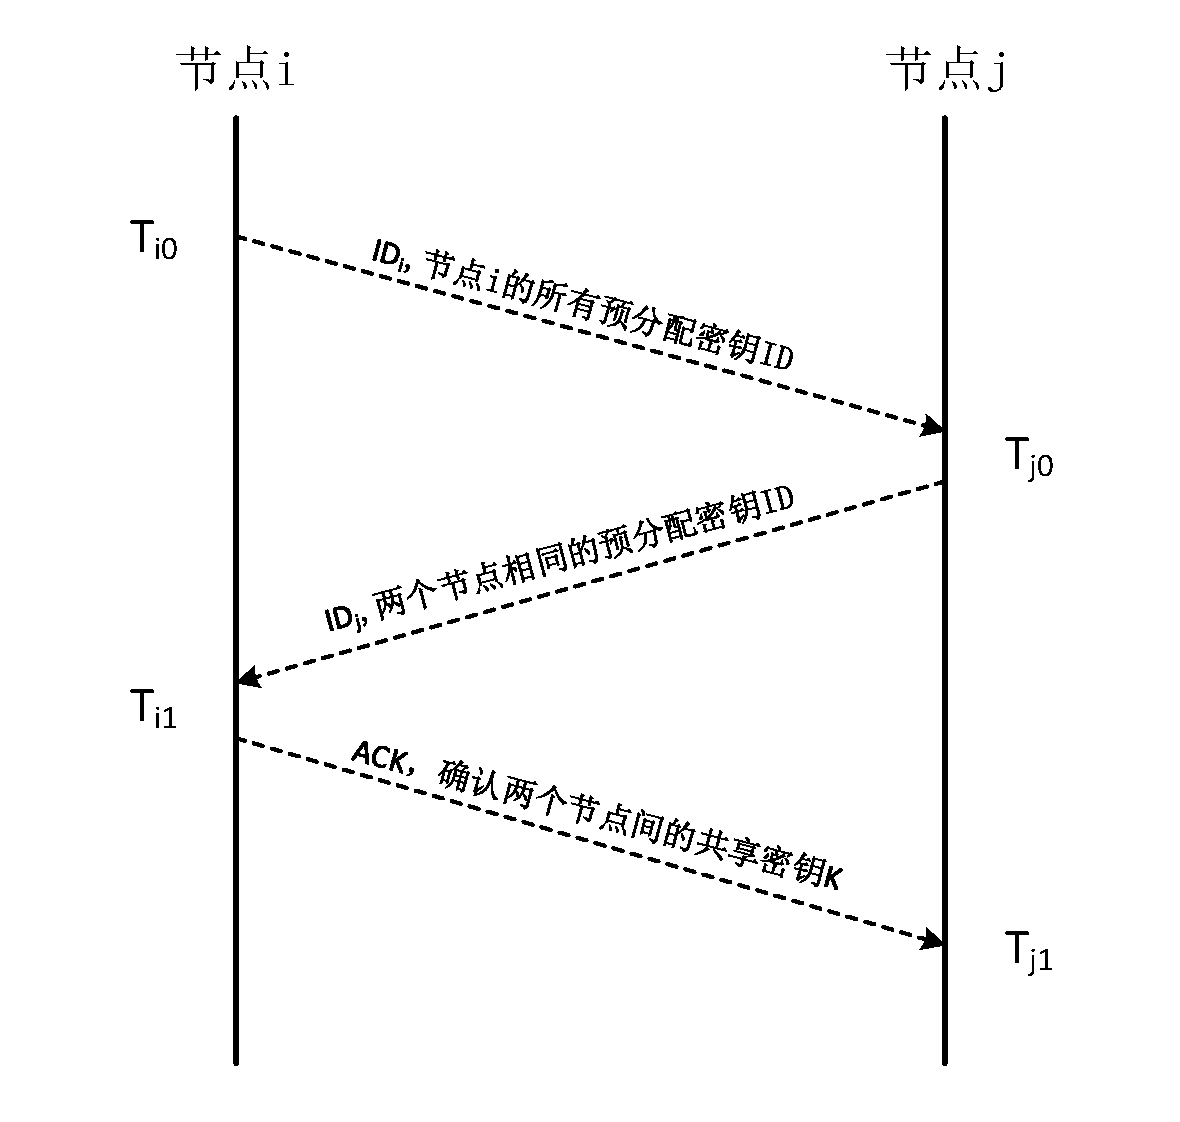
\includegraphics[width=5in]{keyACK}
  \caption{共享密钥建立过程}
  \label{fig:keyACK}
\end{figure}

节点部署到目标区域到网络进行初始化阶段的时间内,假设网络是不受攻击的影响,节点不会被攻击或者被捕获,能安全进行信息的交换。
相邻的节点i与节点j之间发现共享密钥的过程是先由节点i将其节点ID以及所有预分配密钥的ID一起广播。节点j收到邻居节点的ID以及预分配密钥ID以后,在自己的预分配密钥中进行寻找,如果有相同的预分配密钥$K_x$,则将自己的ID以及相同的预分配密钥ID一起发送给节点i。节点i在受到节点j的节点ID和预分配密钥ID后,利用预装配的单向hash函数$H$进行共享密钥的计算:
\begin{equation}
  K=H(<ID_i>\| <ID_j> \|K_x)
\end{equation}
通过将两个节点的节点ID与相同的预分配密钥$K_x$进行拼接以后的单向hash函数计算结果作为两个节点的新共享密钥,这样增强了相邻节点间通信链路的安全性,两个节点的预分配密钥即使因为其他节点被捕获而泄露,攻击者也无法计算出共享密钥$K$,对节点间的通信进行攻击。
\subsubsection{路径密钥发现}
在我们的多跳长路径多节点联合数据认证机制中,通过在路径中发现上下行节点相关关系,对路径中传输的数据报文进行认证。
对于路径密钥,我们使用单向hash函数来进行分配,基站为每个上下行相关节点组生成一个单向hash链作为密钥池,并将这个hash链的密钥种子发送给该相关节点组中距离基站最近的节点。

然后在上下行相关节点组中,每个节点依次使用上行相关节点的路径密钥使用单向hash函数计算自己的路径密钥,$AK_i=H(AK_{i+t})$。通过这样的密钥分配方案,使用了预装配的密钥材料,节约了存储空间的开销,同时单个节点被攻击而被捕获时,丢失的密钥信息较少。
\subsubsection{密钥更新}
无线传感网中,有两种情况需要进行密钥更新:由于无线传感器节点被部署在无人值守区域,容易受到攻击或物理破坏,导致节点失效或者被捕获,攻击者能获取其中的密钥,继而对整个无线传感网进行攻击,所以需要对密钥进行更新;由于无线传感器节点的能量有限,在工作一段时间之后,超过传感器节点的使用期限,需要将失效节点从无线传感网中移除,并对网络中的密钥进行更新。
密钥更新包括两类:

事件触发的更新:无线传感网中有节点能量耗尽而失效时,节点被攻击破坏而失效时都会触发传感网进行密钥的更新。当有新的节点加入传感网,需要同原有节点建立通信链路时也会触发密钥更新。

时间触发的更新:对于基站工作的时间轴,认为一个时间间隔后部分节点的能量可能会耗尽,从而触发密钥更新。新的节点部署到位后,通过共享密钥发现,可以对新加入的节点进行身份认证,保证整个传感网密钥的安全。



\section{消息认证码的实现}
本节讨论适应无线传感网认证需求的消息认证码(Message Authentication code,MAC),首先介绍了集中常见的MAC,然后提出了我们方案中MAC 的设计。

\subsection{消息认证码}
消息认证码是无线传感网中最常见的防数据篡改的工具,利用两个节点之间的共享密钥,对发送的消息进行认证,可以检查消息有没有在传输的过程被篡改。

利用消息认证码通过如下过程来进行认证:发送消息的节点使用共享密钥$K$对消息$M$计算相应的消息认证码$MAC(K,M)$,将$MAC(K,M)$附加在消息报文中发送;当节点接受到该消息报文后,也使用共享密钥$K$对消息$M$计算相应的消息认证码,并与报文中附带的$MAC(K,M)$进行比较,如果相同则说明消息在传输过程中没有被篡改,否则就认为消息已经被篡改。

消息认证码的实现主要可以分为两类:基于hash函数的MAC和基于分组密码的MAC。
\subsubsection{基于hash函数的MAC}
基于hash函数的MAC一般将共享密钥作为hash函数的一个参数,典型的基于hash函数的MAC有HMAC\upcite{c5:hmac}。
%The other efficient, popular candidates include the cascaded-PRF [2], sandwich-MAC [21], and KMDP [14].

HMAC的计算可以表示为$HMAC(K,M)=H((K \oplus opad)\| H((K\oplus ipad)\| M))$,其算法如算法~\ref{alg:hmac}所示:
\begin{algorithm}[htbp]
  \caption{基于带密钥的hash函数的消息认证码HMAC}
  \label{alg:hmac}
  \begin{algorithmic}[1]
    \REQUIRE 输入消息$\mathbf{M}$,认证密钥$\mathbf{K}$,\\
            hash函数$H$,数据块字长$\mathbf{B}$
    \ENSURE 消息认证码HMAC
    \IF{$|\mathbf{K}|>\mathbf{B}$}
        \STATE $K \leftarrow H(K)$
    \ENDIF
    \STATE $\mathbf{K} \leftarrow \mathbf{K}\| (0x00)^{B-|K|}$
    \STATE $ipad \leftarrow (0x36)^\mathbf{B}$
    \STATE $\mathbf{S} \leftarrow H(\mathbf{K}\oplus ipad)\| \mathbf{M})$
    \STATE $opad \leftarrow (0x5c)^\mathbf{B}$
    \STATE $HMAC \leftarrow H(\mathbf{K}\oplus opad)\| \mathbf{S})$
  \end{algorithmic}
\end{algorithm}

\subsubsection{基于分组密码的MAC}
基于分组密码的MAC最早的方案是CBC-MAC,
作者又在CBC-MAC方案的基础上增加了计算的并行性,提出了XOR-MAC方案
\upcite{c5:xormac}。
XOR-MAC可以分为随机异或MAC方案(XMACR)和基于计数器异或方案(XMACC)。

随机异或MAC方案(XMACR)的算法和基于计数器异或方案(XMACC)的算法分别如算法~\ref{alg:xormacA}和算法~\ref{alg:xormacB}所示:
\begin{algorithm}[htbp]
  \caption{XMACR}
  \label{alg:xormacA}
  \begin{algorithmic}[1]
    \REQUIRE 输入消息$\mathbf{M}$,认证密钥$\mathbf{K}$,\\
            分组密码$E:k\times \{0,1\}^n \rightarrow \{0,1\}^n$
    \ENSURE 消息认证码
    \STATE $M \leftarrow M\| 1\|0^t$,将M填充为$n-b-1$的整数倍
    \IF{$|M|\leq (n-b-1)2^b$}
        \STATE 将消息M分隔为$M_1,M_2,\cdots,M_m$
    \ENDIF
    \STATE $r \leftarrow \{0,1\}^{n-1}$
    \STATE $y_0\leftarrow E_K(0\|r)$
    \FOR{$i=1$ to $m$}
        \STATE $y_i \leftarrow y_{i-1}\oplus E_K(1\|<i>\|M_i)$
    \ENDFOR
    \RETURN $r,y_m$
  \end{algorithmic}
\end{algorithm}


\begin{algorithm}[htbp]
  \caption{XMACC}
  \label{alg:xormacB}
  \begin{algorithmic}[1]
    \REQUIRE 输入消息$\mathbf{M}$,认证密钥$\mathbf{K}$,\\
            分组密码$E:k\times \{0,1\}^n \rightarrow \{0,1\}^n$
    \ENSURE 消息认证码
    \STATE $M \leftarrow M\| 1\|0^t$,将M填充为$n-b-1$的整数倍
    \IF{$|M|\leq (n-b-1)2^b$}
        \STATE 将消息M分隔为$M_1,M_2,\cdots,M_m$
    \ENDIF
    \STATE $counter \leftarrow counter+1$
    \STATE $y_0\leftarrow E_K(0\|<counter>)$
    \FOR{$i=1$ to $m$}
        \STATE $y_i \leftarrow y_{i-1}\oplus E_K(1\|<i>\|M_i)$
    \ENDFOR
    \RETURN $counter,y_m$
  \end{algorithmic}
\end{algorithm}

\subsection{MAC设计实现}

使用XOR-MAC等方案虽然增加了并行性,对计算长消息的MAC有较好的效率,但是这些算法使用了密钥扩展,多次调用伪随机函数,导致计算短消息时开销过大。
由于CBC-MAC等方案对长度扩展攻击的防御不够好,我们在其基础上进行了改进,提出了SCBC-MAC方案。
SCBC方案的计算过程如图~\ref{fig:scbc}所示:

\begin{figure}[htbp]
  \centering
  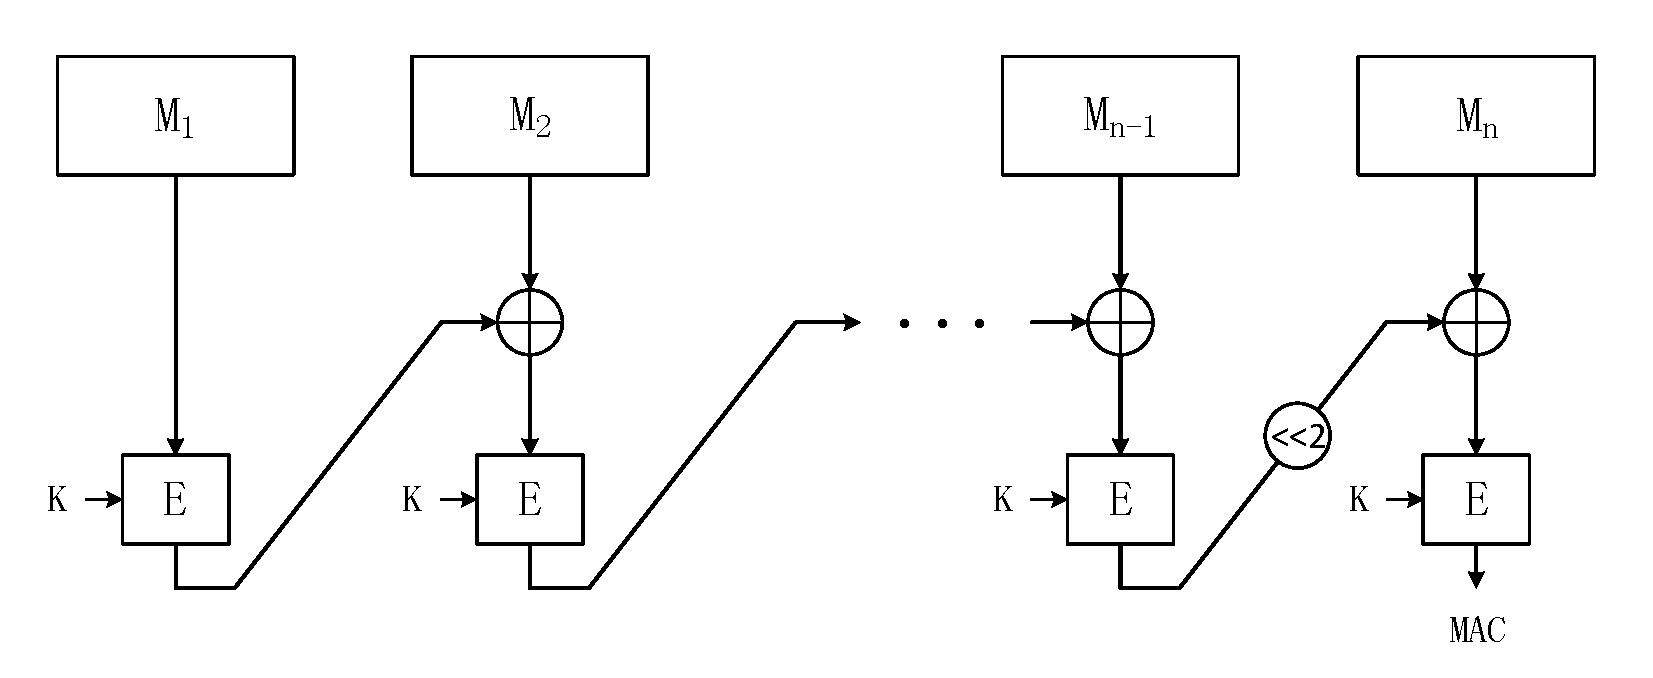
\includegraphics[width=5in]{scbc}
  \caption{SCBC-MAC方案}
  \label{fig:scbc}
\end{figure}

通过对消息$M$进行填充$M\| 1\|0^t$,使得消息M可以表示为$M=(M_1\|M_2\| \cdots \| M_n)\in (\{0,1\}^l)^n,l\geq 2$。我们的SCBC-MAC方案计算MAC可以表示如下:
\begin{equation}\label{scbc}
  SCBC_K(M)=E_K(E_K(\cdots E_K(E_K(M_1)\oplus M_2) \cdots)\ll 2 \oplus M_n)
\end{equation}

我们通过在最后一个消息块进行XOR运算之前,增加了一个左移2位的操作,这样简单的调整有效阻止了长度扩展攻击。SCBC-MAC的算法可以表示为算法~\ref{alg:scbc-mac}:

\begin{algorithm}[htbp]
  \caption{SCBC-MAC}
  \label{alg:scbc-mac}
  \begin{algorithmic}[1]
    \REQUIRE 输入消息$\mathbf{M}$,认证密钥$\mathbf{K}$,\\
            分组密码$E:k\times \{0,1\}^n \rightarrow \{0,1\}^n$
    \ENSURE 消息认证码
    \STATE $M \leftarrow M\| 1\|0^t$,将M填充为$l$的整数倍
    \IF{$l\geq 2$}
        \STATE 将消息M分隔为$M_1,M_2,\cdots,M_n$
    \ENDIF
    \STATE $y_0\leftarrow 0^l$
    \FOR{$i=1$ to $n-1$}
        \STATE $y_i \leftarrow y_{i-1}\oplus E_K(M_i)$
    \ENDFOR
    \STATE $y_n \leftarrow E_K(y_{n-1}\ll 2 \oplus E_K(M_n))$
    \RETURN $y_n$
  \end{algorithmic}
\end{algorithm}


\section{本章小结}
本章主要完成了密钥分配方案和消息认证码的设计。针对数据认证中的密钥分配需求,我们设计实现了基于单向hash链的密钥分配方案。对于报文传输阶段中使用的消息认证码,我们介绍了多种MAC方案,并针对我们的数据认证机制需求设计了SCBC-MAC方案。
